\section{Diagnostic Flip Coverage}
\label{sec:repair}

\paragraph{30.1 Component improvements.} The repair is diagnostic, not a
product: training on oracle-mined boundary-crossing variations (flipmine)
tests whether exposing the model to the missing update shape changes
behavior. On the fresh holdout: single-flip C1 miss $52.4\% \to 34.7\%$
(paired same-sample comparison; C0 false alarm $26.2\% \to 23.8\%$, within
$\pm 5$pp, so no alarm inflation); action invalid at $\lambda{=}2$,
$75.0\% \to 62.5\%$; turn miss $43.8\% \to 31.3\%$; and static error
\emph{improves}, $18.0\% \to 10.7\%$. The U02 decision-interface
decomposition locates much of the action gain in coverage (feasible-set size
$3.6\times$) that persists across score, lexicographic, and calibrated
rules, while temperature rescaling at fixed threshold is provably a no-op
on the feasible set (calibrated $\equiv$ lexicographic by construction) and
fitted temperatures ($T{=}8.1$ clean / $8.4$ flipmine) show ordinary
overconfidence, corrected after a sign fix that invalidated an earlier
``anti-information'' reading. Decomposed by decision interface, repair
gains separate into genuine component capability (static, single-flip,
candidate recall and ranking, which an affine rescaling of clean logits
cannot reproduce) and operating-point shifts (action coverage), with the
split depending on the interface (Sec.~7).

\paragraph{30.2 Endpoint repair is not full repair.} Targeted flip coverage
improves several component and downstream metrics, but paired quartet
analysis reveals that endpoint repair substantially overstates recovery of
full compositional consistency. On baseline-110 quartets (both atomics
correct, AB wrong under clean), full repair ($110 \to 111$) is only
$0.03$--$0.10$ while error migration---AB correct \emph{but} an atomic newly
wrong---is $0.36$--$0.40$ (parent-cluster CIs; Fig.~3). Joint consistency
$J = P(111)$ barely moves ($0.05$--$0.06 \to 0.06$--$0.08$), and on the
common-correct set the repair direction is inconsistent across seeds
(including one reversal). A preserve-balanced retraining pilot with matched
loss weights does not reduce migration. Core sentence: most endpoint gains do not restore the original atomic
competencies jointly with the composed outcome (Fig.~\ref{fig:migration}).

\begin{figure}[t]
\centering
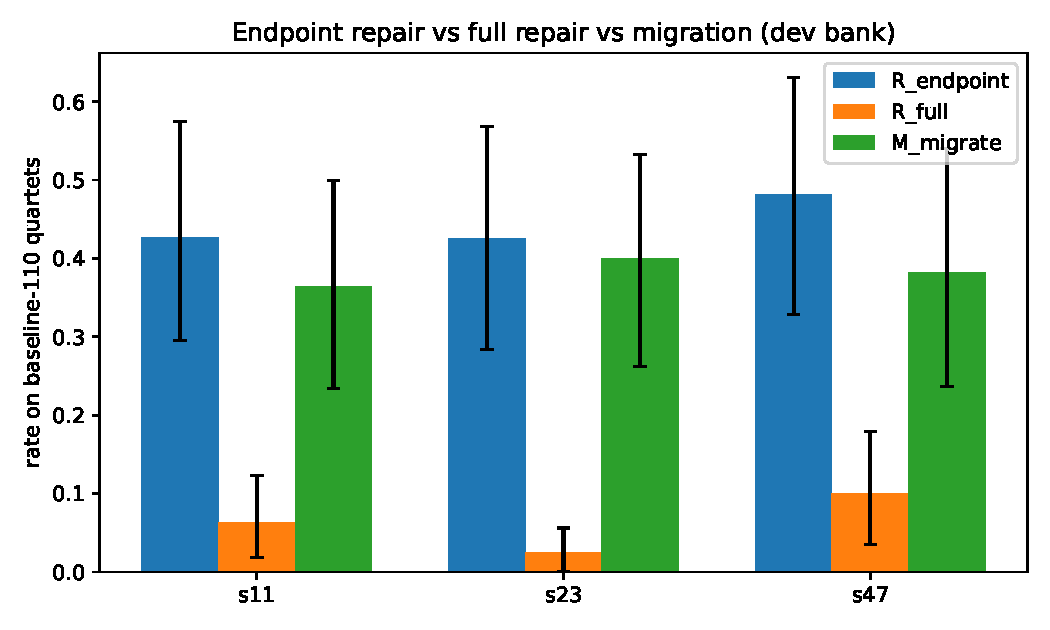
\includegraphics[width=0.9\linewidth]{../figures/fig3_p3_migration.pdf}
\caption{Endpoint repair vs full repair vs error migration on baseline-110
quartets (dev bank, parent-cluster intervals). Most gains migrate.}
\label{fig:migration}
\end{figure}

\paragraph{30.3 Representation lead: relational features.} Explicit
label-free relational input features change the picture where flip coverage
alone could not: joint consistency rises to $0.13$--$0.21$ (dev) and
$0.16$--$0.23$ (fresh parent-disjoint confirmation), $3/3$ seeds, with mean
$\Delta J \ge 5$pp and \emph{improved} static accuracy ($0.15$--$0.17 \to
0.06$), so the gain is not bought by static degradation. Combined
relational-plus-flip training reaches $J$ $0.38$--$0.47$ with full repair $0.45$--$0.50$ exceeding migration $0.25$--$0.30$ on confirmation---the
reverse of the raw-flipmine pattern. This suggests the representation of
relations, not simply additional flip coverage, matters for preserving
atomic and joint correctness together. The features are hand-designed and
relation-aware by construction; we claim an existence proof for joint
consistency, not a general architecture principle, and open no further
relation-architecture search.
